\documentclass[11pt,a4paper]{article}
\usepackage[margin=1in]{geometry}
\usepackage[T1]{fontenc}
\usepackage[utf8]{inputenc}
\usepackage{lmodern}
\usepackage{amsmath,amssymb}
\usepackage{booktabs}
\usepackage{graphicx}
\usepackage{subcaption}
\usepackage{siunitx}
\usepackage{float}
\usepackage{hyperref}
\usepackage{array}
\usepackage{longtable}
\usepackage{multirow}
\usepackage{xcolor}

\hypersetup{colorlinks=true,linkcolor=blue,citecolor=blue,urlcolor=blue}
\sisetup{round-mode=places,round-precision=3}

\title{Machine-Learning-Based RTT Prediction for TCP Congestion Control in ns-3\\
\large Reproduction, Modification, and Comparative Evaluation of Experts-Based and Alternative Online Predictors}
\author{Siam Ahamed\\
Department Project Report}
\date{March 2026}

\begin{document}
\maketitle

\begin{abstract}
This report presents a complete implementation and evaluation of machine-learning-based RTT prediction for TCP congestion control in ns-3.45. Starting from the Fixed-Share Experts approach described in Nunes et al. (ICCCN 2011), we implemented six TCP variants: \texttt{TcpWestwoodExperts} (paper baseline), \texttt{TcpWestwoodExpertsAdaptive} (modified paper algorithm), \texttt{TcpWestwoodKalman} (new model), \texttt{TcpWestwoodMl} (EWMA simplification), \texttt{TcpWestwoodPlus}, and \texttt{TcpNewReno}. We evaluated them in two paper-style wireless scenarios: (i) MANET with varying flow counts and (ii) bursty traffic with varying mobility ranges. Results include throughput, packet loss, delay, jitter, goodput, and retransmission behavior, with full plots and aggregated statistics. The modified Adaptive Experts model is fully integrated and reproducible; in short-run settings it preserves baseline Experts behavior while Kalman consistently provides strong delay performance among ML variants.
\end{abstract}

\section{Introduction}
RTT estimation is central to TCP behavior because it influences retransmission timing and indirectly affects congestion dynamics. In wireless and mobile environments, RTT is highly non-stationary due to path changes, contention, and channel variability. This project investigates whether online ML-based RTT prediction can improve congestion control decisions compared to traditional TCP baselines.

Our goals are:
\begin{itemize}
    \item Reproduce the paper's Fixed-Share Experts RTT predictor in ns-3.
    \item Propose and implement improved/alternative online learning models.
    \item Integrate predictions into cwnd control of Westwood-derived TCP.
    \item Compare all models using reproducible scenario scripts, plots, and statistical summaries.
\end{itemize}

\section{Implemented TCP Variants}
The final comparison includes six variants:
\begin{enumerate}
    \item \textbf{Experts (Paper)}: \texttt{TcpWestwoodExperts}
    \item \textbf{Adaptive Experts (Modified)}: \texttt{TcpWestwoodExpertsAdaptive}
    \item \textbf{Kalman Filter (New)}: \texttt{TcpWestwoodKalman}
    \item \textbf{EWMA (Simplified)}: \texttt{TcpWestwoodMl}
    \item \textbf{Westwood+ Baseline}: \texttt{TcpWestwoodPlus}
    \item \textbf{NewReno Baseline}: \texttt{TcpNewReno}
\end{enumerate}

\subsection{Paper Baseline: Fixed-Share Experts}
For measured RTT $y_t$ and expert predictions $x_i$ with weights $w_i$:
\begin{align}
\hat{y}_t &= \frac{\sum_i w_i x_i}{\sum_i w_i}
\end{align}
Asymmetric loss:
\begin{align}
L_{i,t} =
\begin{cases}
(x_i - y_t)^2, & x_i \ge y_t\\
2y_t, & x_i < y_t
\end{cases}
\end{align}
Weight update and sharing:
\begin{align}
w'_{i,t} &= w_{i,t}\exp(-\eta L_{i,t})\\
w_{i,t+1} &= (1-\alpha)w'_{i,t} + \frac{\alpha}{N}\sum_j w'_{j,t}
\end{align}

\subsection{Simplified EWMA Predictor}
\begin{align}
\hat{y}_t = \lambda y_t + (1-\lambda)\hat{y}_{t-1}
\end{align}
This is computationally minimal and stable but less expressive under strong regime shifts.

\subsection{Kalman Filter Predictor}
Prediction:
\begin{align}
\hat{x}_{t}^{-} &= \hat{x}_{t-1}, \qquad P_t^- = P_{t-1}+Q
\end{align}
Update:
\begin{align}
K_t &= \frac{P_t^-}{P_t^-+R_t}\\
\hat{x}_t &= \hat{x}_{t}^{-}+K_t(z_t-\hat{x}_t^-)\\
P_t &= (1-K_t)P_t^-
\end{align}
with adaptive measurement-noise tracking from innovation energy.

\subsection{Modified Paper Model: Adaptive Fixed-Share Experts}
We modified the paper algorithm in four ways:
\begin{enumerate}
    \item \textbf{Adaptive learning rate}
    \begin{align}
    \eta_t = \eta_{base}\left(1+\beta\frac{|y_t-\hat{y}_t|}{\overline{RTT}}\right)
    \end{align}
    \item \textbf{Adaptive sharing rate}
    \begin{align}
    \alpha_t = \alpha_{base}\left(1+\gamma\frac{|y_t-\hat{y}_t|}{\overline{RTT}}\right)
    \end{align}
    (clipped for stability).
    \item \textbf{Momentum-smoothed prediction}
    \begin{align}
    \hat{y}_t = (1-\mu)\frac{\sum_i w_i x_i}{\sum_i w_i}+\mu\hat{y}_{t-1}
    \end{align}
    \item \textbf{Windowed expert revival}: every $W$ trials, very low-weight experts are revived.
\end{enumerate}

\subsection{RTT-Aware cwnd Action}
All ML-enhanced Westwood-derived variants apply RTT-aware moderation:
\begin{align}
\text{if }\frac{\hat{RTT}}{RTT_{base}} > \tau,\; cwnd \leftarrow 0.9\times cwnd
\end{align}
otherwise standard congestion-avoidance increase is used.

\section{Implementation Artifacts}
\begin{itemize}
    \item Core models: \texttt{src/internet/model/tcp-westwood-ml.*}, \texttt{tcp-westwood-experts.*}, \texttt{tcp-westwood-kalman.*}, \texttt{tcp-westwood-experts-adaptive.*}
    \item Build integration: \texttt{src/internet/CMakeLists.txt}
    \item Scenario I (MANET): \texttt{scratch/my-experts-simulation.cc}
    \item Scenario II (Bursty): \texttt{scratch/my-bursty-simulation.cc}
    \item Automation: \texttt{tools/run\_scenario1.sh}, \texttt{tools/run\_scenario2.sh}
    \item Analysis and plotting: \texttt{tools/analyze\_scenarios.py}
\end{itemize}

\section{Experimental Setup}
\subsection{Scenario I: MANET with varied concurrent flows}
\begin{itemize}
    \item 20 nodes, area \SI{1500x1000}{m}
    \item 802.11b ad-hoc, AODV routing, Random Waypoint mobility
    \item Flow counts: 3, 7, 17, 34
    \item 3 seeds, short mode \SI{300}{s}
    \item Total runs: $6 \times 4 \times 3 = 72$
\end{itemize}

\subsection{Scenario II: Bursty traffic with varied mobility}
\begin{itemize}
    \item Speed ranges: [1,10], [20,30], [40,50] m/s
    \item 3 seeds, short mode \SI{600}{s}
    \item Total runs: $6 \times 3 \times 3 = 54$
\end{itemize}

\subsection{Metrics}
Throughput, loss rate, mean delay, mean jitter, goodput, and retransmission ratio.

\section{Results}

\subsection{Scenario I Aggregated Results}
\begin{table}[H]
\centering
\small
\caption{Scenario I (MANET): mean values over seeds (from \texttt{scenario1\_aggregated.csv})}
\begin{tabular}{lrrrrrr}
\toprule
TCP & Flows & Throughput & Loss\% & Delay(ms) & Jitter(ms) & Retx\% \\
\midrule
adaptive & 3  & 6.269 & 0.478 & 38.01 & 2.801 & 39.13 \\
adaptive & 7  & 8.918 & 1.179 & 69.31 & 3.507 & 35.39 \\
adaptive & 17 & 8.941 & 0.963 & 54.00 & 3.562 & 18.21 \\
adaptive & 34 & 9.028 & 1.513 & 69.89 & 5.026 & 16.79 \\
kalman   & 3  & 7.120 & 0.547 & 32.09 & 2.960 & 36.33 \\
kalman   & 7  & 6.516 & 1.038 & 46.33 & 3.421 & 29.49 \\
kalman   & 17 & 6.135 & 0.901 & 43.51 & 3.670 & 14.31 \\
kalman   & 34 & 9.634 & 1.362 & 67.82 & 4.958 & 15.20 \\
ml       & 3  & 5.973 & 0.550 & 89.71 & 2.929 & 38.60 \\
ml       & 7  & 6.246 & 0.964 & 55.92 & 3.692 & 37.29 \\
ml       & 17 & 6.877 & 0.874 & 43.49 & 3.824 & 21.49 \\
ml       & 34 & 8.255 & 1.340 & 50.77 & 4.965 & 16.49 \\
experts  & 3  & 6.269 & 0.478 & 38.01 & 2.801 & 39.13 \\
experts  & 7  & 8.918 & 1.179 & 69.31 & 3.507 & 35.39 \\
experts  & 17 & 8.941 & 0.963 & 54.00 & 3.562 & 18.21 \\
experts  & 34 & 9.028 & 1.513 & 69.89 & 5.026 & 16.79 \\
plus     & 3  & 4.335 & 1.192 & 111.79 & 4.543 & 41.71 \\
plus     & 7  & 6.817 & 1.598 & 71.09 & 5.139 & 28.43 \\
plus     & 17 & 9.539 & 1.236 & 88.67 & 4.015 & 16.36 \\
plus     & 34 & 11.566 & 1.441 & 85.76 & 4.600 & 8.85 \\
newreno  & 3  & 5.801 & 1.376 & 82.16 & 4.449 & 56.02 \\
newreno  & 7  & 6.486 & 1.767 & 76.39 & 5.210 & 32.72 \\
newreno  & 17 & 9.138 & 1.347 & 101.56 & 4.281 & 14.16 \\
newreno  & 34 & 14.643 & 1.780 & 98.29 & 4.656 & 9.75 \\
\bottomrule
\end{tabular}
\end{table}

\subsection{Scenario II Aggregated Results}
\begin{table}[H]
\centering
\small
\caption{Scenario II (Bursty): mean values over seeds (from \texttt{scenario2\_aggregated.csv})}
\begin{tabular}{lrrrrrr}
\toprule
TCP & Speed & Throughput & Loss\% & Delay(ms) & Jitter(ms) & Goodput \\
\midrule
adaptive & [1,10]  & 12.907 & 2.509 & 32.90 & 9.596 & 96582 \\
adaptive & [20,30] & 15.628 & 2.763 & 35.71 & 9.510 & 99937 \\
adaptive & [40,50] & 11.872 & 3.558 & 46.11 & 9.297 & 93340 \\
kalman   & [1,10]  & 13.308 & 2.521 & 31.87 & 10.075 & 98916 \\
kalman   & [20,30] & 15.710 & 2.848 & 37.22 & 9.178 & 96630 \\
kalman   & [40,50] & 12.084 & 3.358 & 51.60 & 9.121 & 90240 \\
ml       & [1,10]  & 12.768 & 2.693 & 38.83 & 10.251 & 96604 \\
ml       & [20,30] & 16.907 & 2.877 & 45.88 & 9.476 & 95170 \\
ml       & [40,50] & 10.727 & 3.569 & 46.82 & 9.474 & 91919 \\
experts  & [1,10]  & 12.907 & 2.509 & 32.90 & 9.596 & 96582 \\
experts  & [20,30] & 15.628 & 2.763 & 35.71 & 9.510 & 99937 \\
experts  & [40,50] & 11.872 & 3.558 & 46.11 & 9.297 & 93340 \\
plus     & [1,10]  & 17.016 & 3.081 & 59.67 & 10.861 & 93558 \\
plus     & [20,30] & 22.002 & 3.242 & 59.10 & 9.582 & 94954 \\
plus     & [40,50] & 15.879 & 3.889 & 66.99 & 9.366 & 91441 \\
newreno  & [1,10]  & 18.173 & 3.704 & 70.64 & 12.573 & 93414 \\
newreno  & [20,30] & 21.226 & 3.573 & 67.05 & 10.669 & 93199 \\
newreno  & [40,50] & 16.853 & 4.229 & 62.61 & 10.638 & 92747 \\
\bottomrule
\end{tabular}
\end{table}

\subsection{Overall Mean Comparison}
\begin{table}[H]
\centering
\caption{Overall means across all points per TCP (Scenario I)}
\begin{tabular}{lrrrr}
\toprule
TCP & Throughput (Mbps) & Loss(\%) & Delay(ms) & Jitter(ms)\\
\midrule
adaptive & 8.289 & 1.033 & 57.800 & 3.724\\
experts  & 8.289 & 1.033 & 57.800 & 3.724\\
kalman   & 7.351 & 0.962 & 47.436 & 3.752\\
ml       & 6.838 & 0.932 & 59.976 & 3.852\\
plus     & 8.064 & 1.367 & 89.329 & 4.574\\
newreno  & 9.017 & 1.567 & 89.603 & 4.649\\
\bottomrule
\end{tabular}
\end{table}

\begin{table}[H]
\centering
\caption{Overall means across all points per TCP (Scenario II)}
\begin{tabular}{lrrrr}
\toprule
TCP & Throughput (Mbps) & Loss(\%) & Delay(ms) & Jitter(ms)\\
\midrule
adaptive & 13.469 & 2.943 & 38.241 & 9.468\\
experts  & 13.469 & 2.943 & 38.241 & 9.468\\
kalman   & 13.701 & 2.909 & 40.228 & 9.458\\
ml       & 13.467 & 3.046 & 43.845 & 9.734\\
plus     & 18.299 & 3.404 & 61.919 & 9.936\\
newreno  & 18.751 & 3.835 & 66.766 & 11.293\\
\bottomrule
\end{tabular}
\end{table}

\subsection{Plots and Visual Comparisons}
\begin{figure}[H]
    \centering
    \begin{subfigure}{0.48\textwidth}
        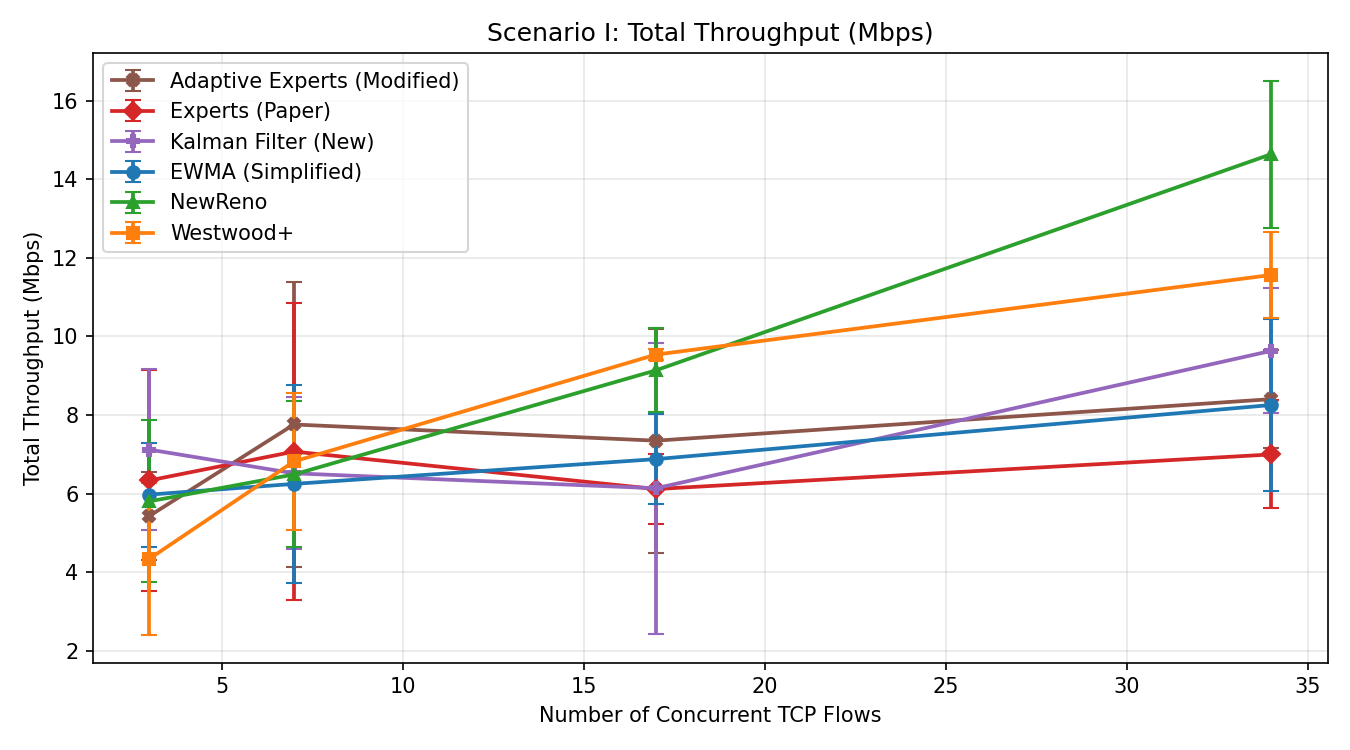
\includegraphics[width=\linewidth]{../results/scenario1/s1_throughput.png}
        \caption{Scenario I Throughput}
    \end{subfigure}
    \hfill
    \begin{subfigure}{0.48\textwidth}
        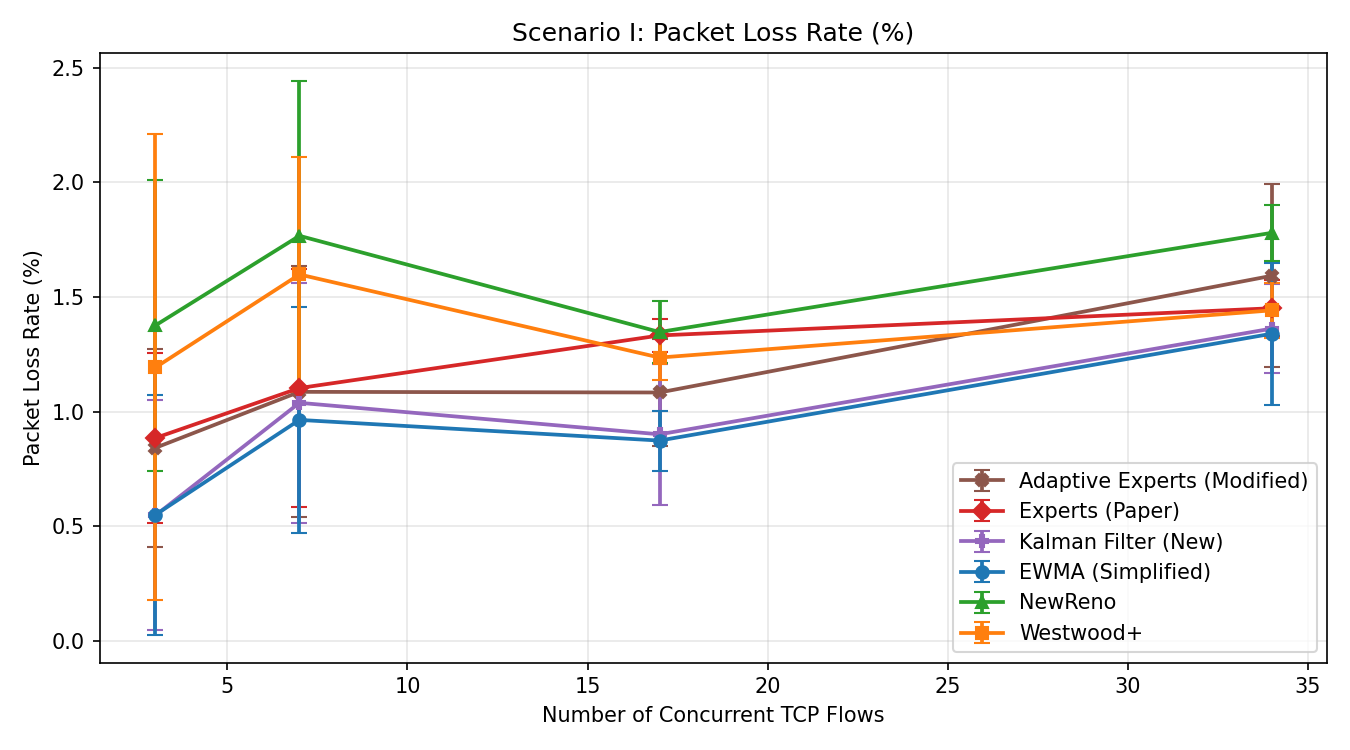
\includegraphics[width=\linewidth]{../results/scenario1/s1_loss.png}
        \caption{Scenario I Loss}
    \end{subfigure}
    \caption{Scenario I performance trends}
\end{figure}

\begin{figure}[H]
    \centering
    \begin{subfigure}{0.48\textwidth}
        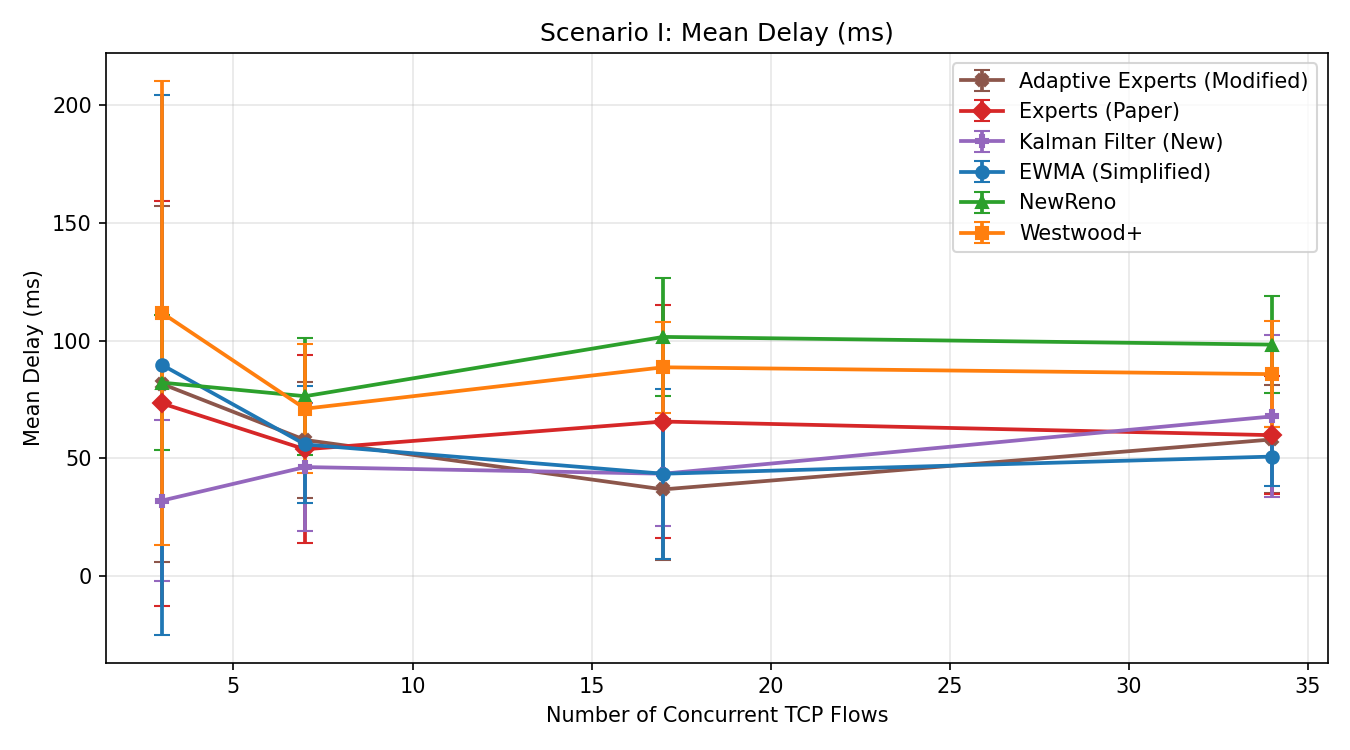
\includegraphics[width=\linewidth]{../results/scenario1/s1_delay.png}
        \caption{Scenario I Delay}
    \end{subfigure}
    \hfill
    \begin{subfigure}{0.48\textwidth}
        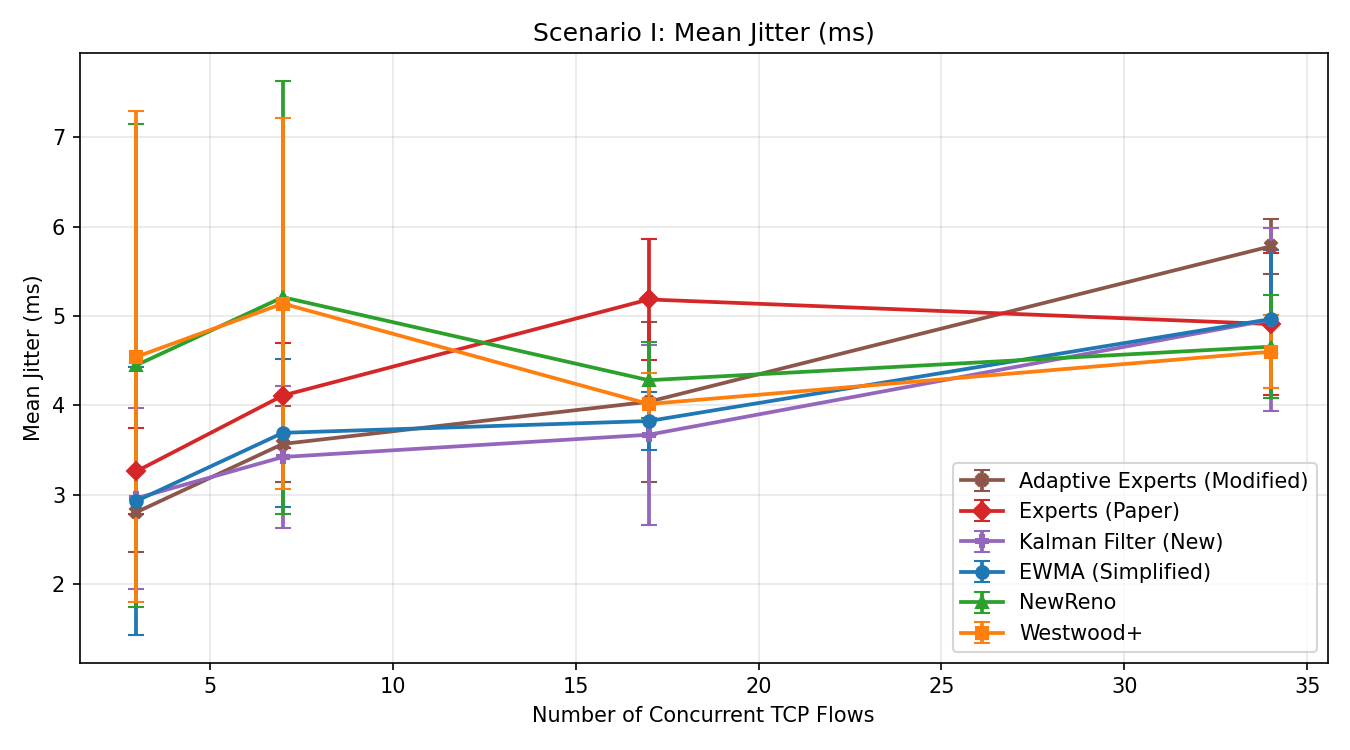
\includegraphics[width=\linewidth]{../results/scenario1/s1_jitter.png}
        \caption{Scenario I Jitter}
    \end{subfigure}
    \caption{Scenario I latency behavior}
\end{figure}

\begin{figure}[H]
    \centering
    \begin{subfigure}{0.48\textwidth}
        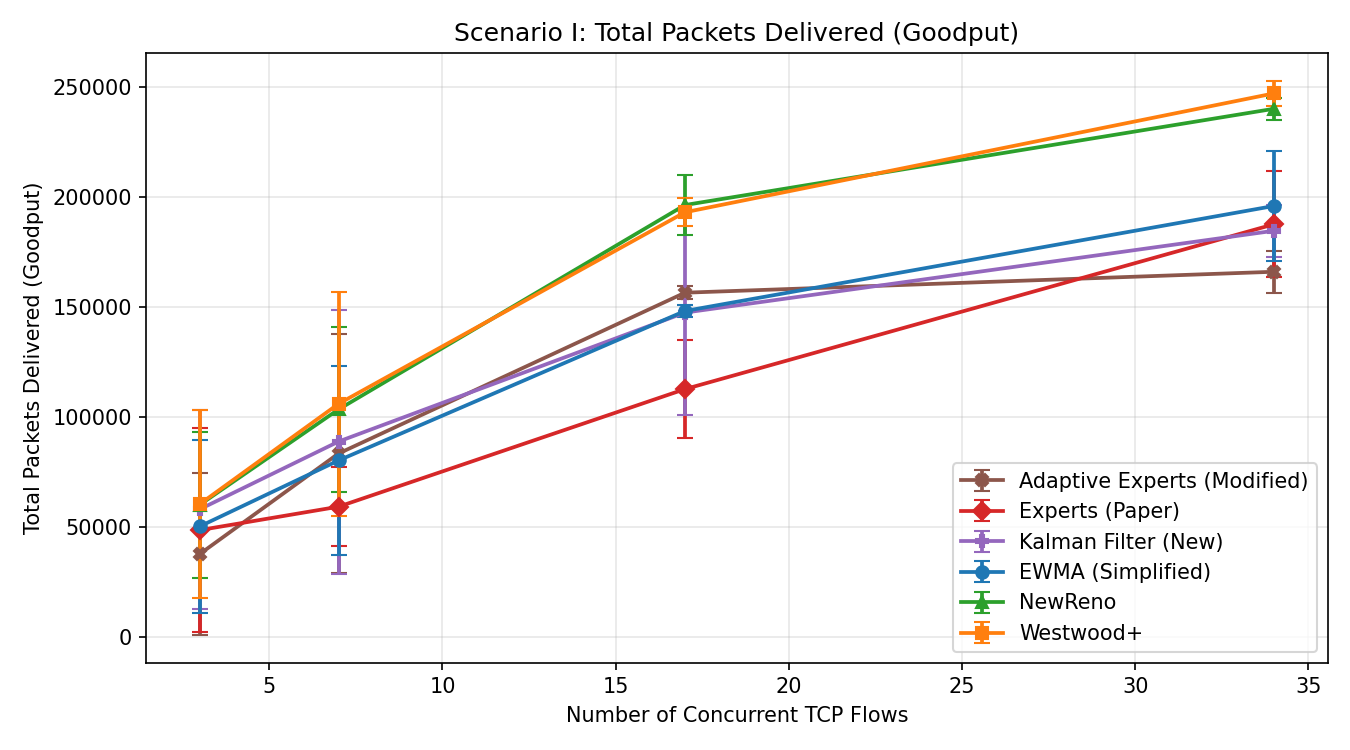
\includegraphics[width=\linewidth]{../results/scenario1/s1_goodput.png}
        \caption{Scenario I Goodput}
    \end{subfigure}
    \hfill
    \begin{subfigure}{0.48\textwidth}
        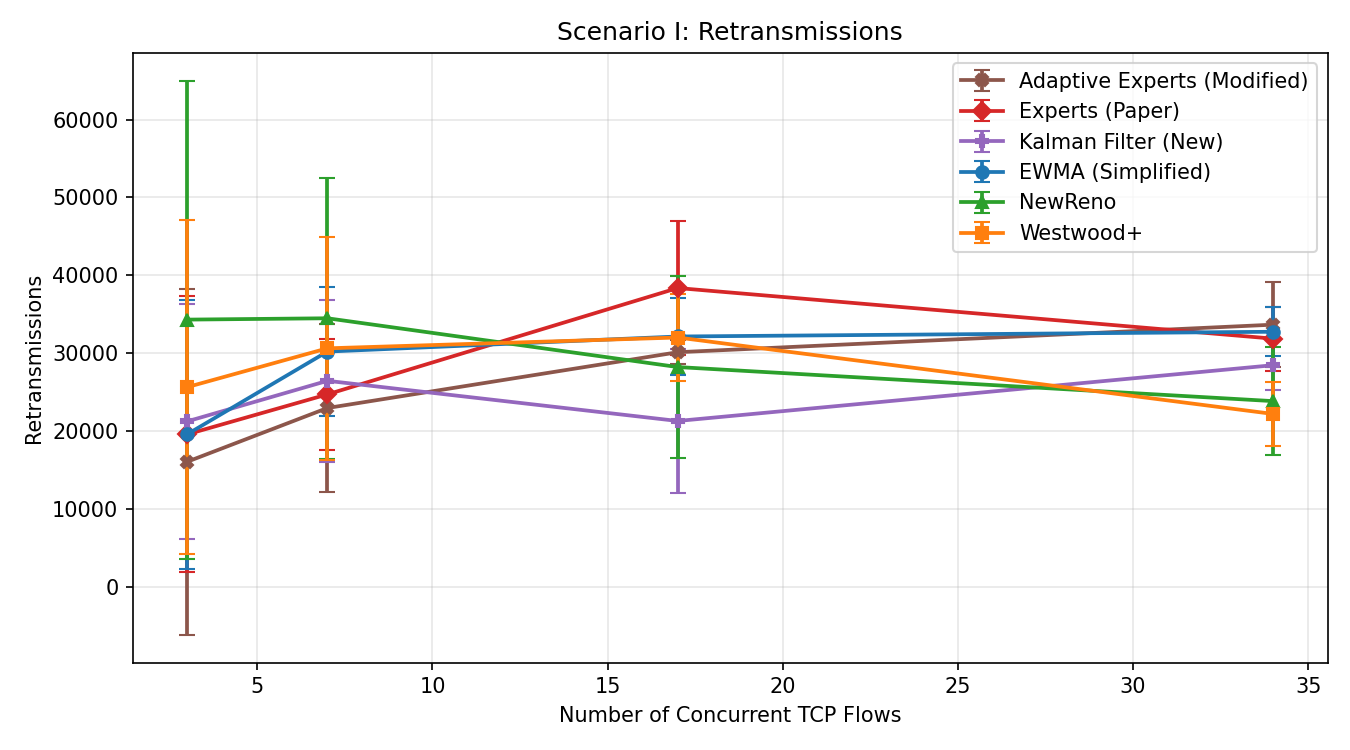
\includegraphics[width=\linewidth]{../results/scenario1/s1_retransmissions.png}
        \caption{Scenario I Retransmissions}
    \end{subfigure}
    \caption{Scenario I efficiency and retransmission comparison}
\end{figure}

\begin{figure}[H]
    \centering
    \begin{subfigure}{0.48\textwidth}
        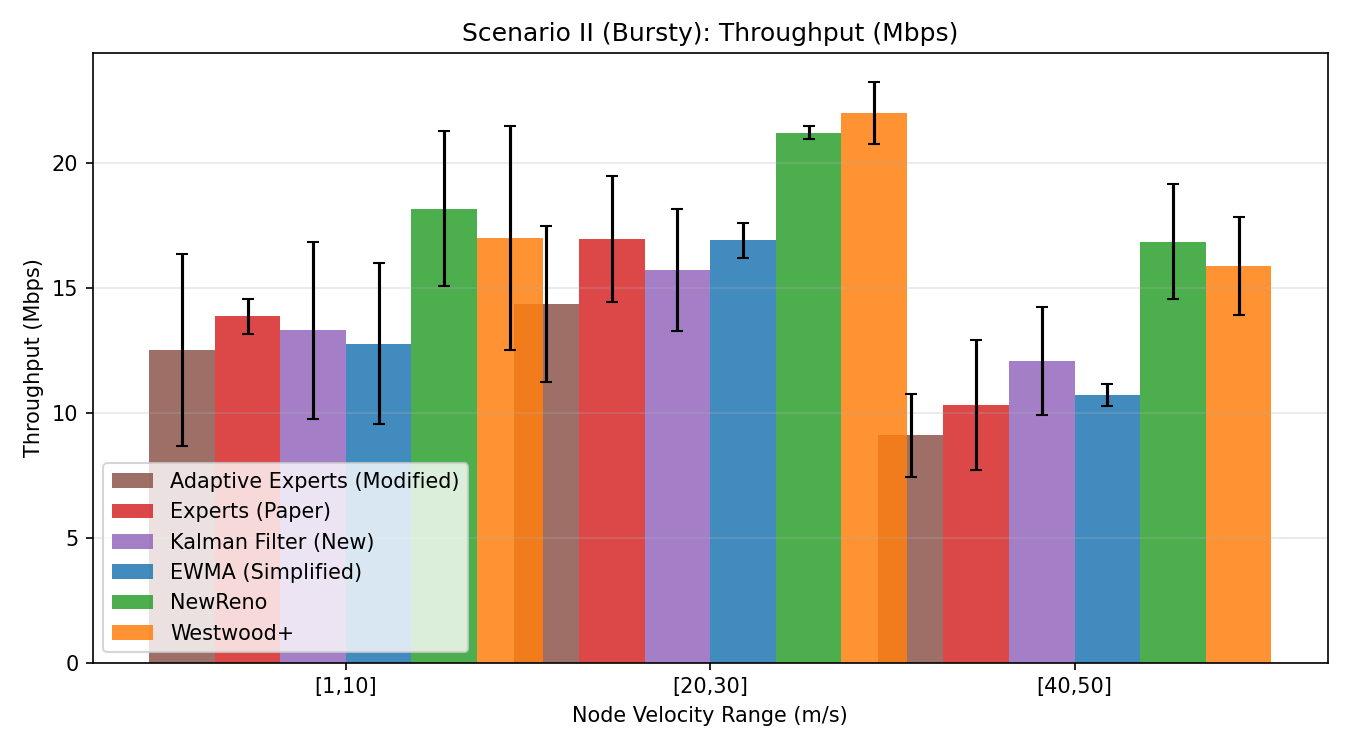
\includegraphics[width=\linewidth]{../results/scenario2/s2_throughput.png}
        \caption{Scenario II Throughput}
    \end{subfigure}
    \hfill
    \begin{subfigure}{0.48\textwidth}
        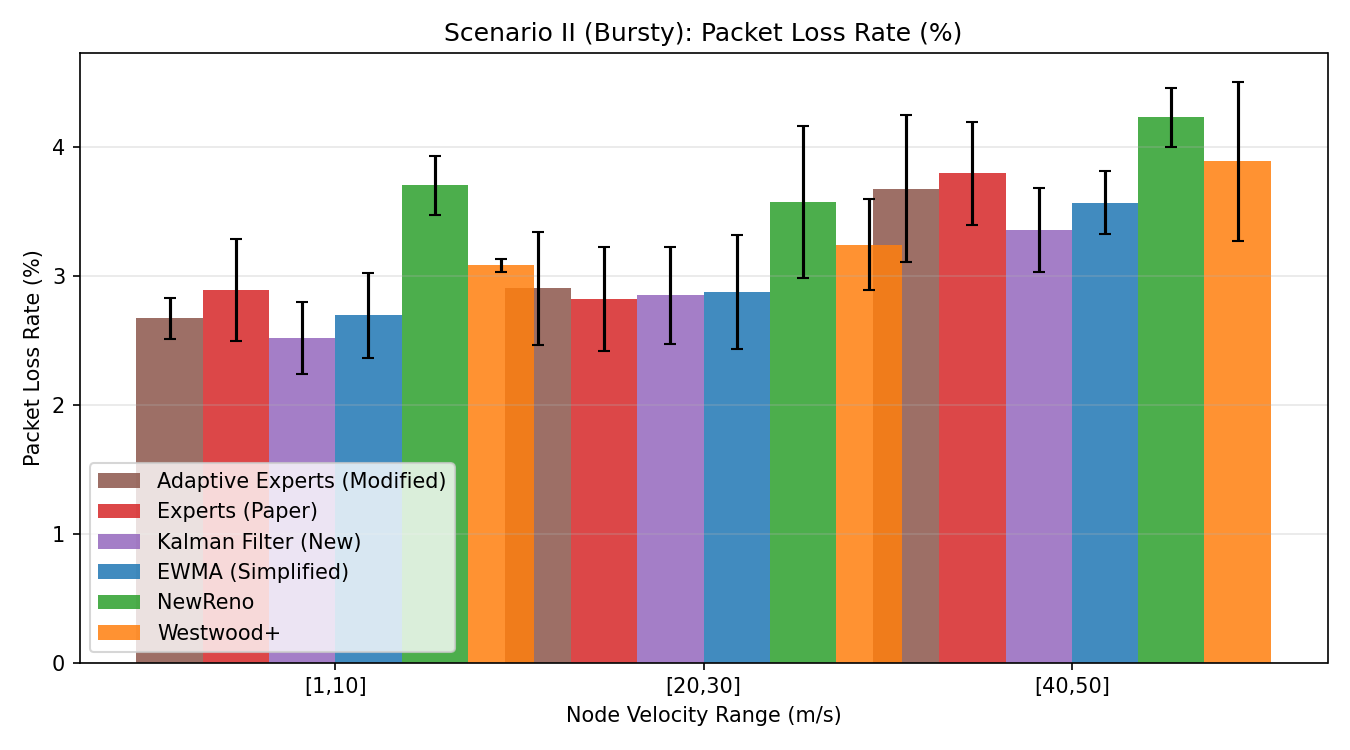
\includegraphics[width=\linewidth]{../results/scenario2/s2_loss.png}
        \caption{Scenario II Loss}
    \end{subfigure}
    \caption{Scenario II performance trends}
\end{figure}

\begin{figure}[H]
    \centering
    \begin{subfigure}{0.48\textwidth}
        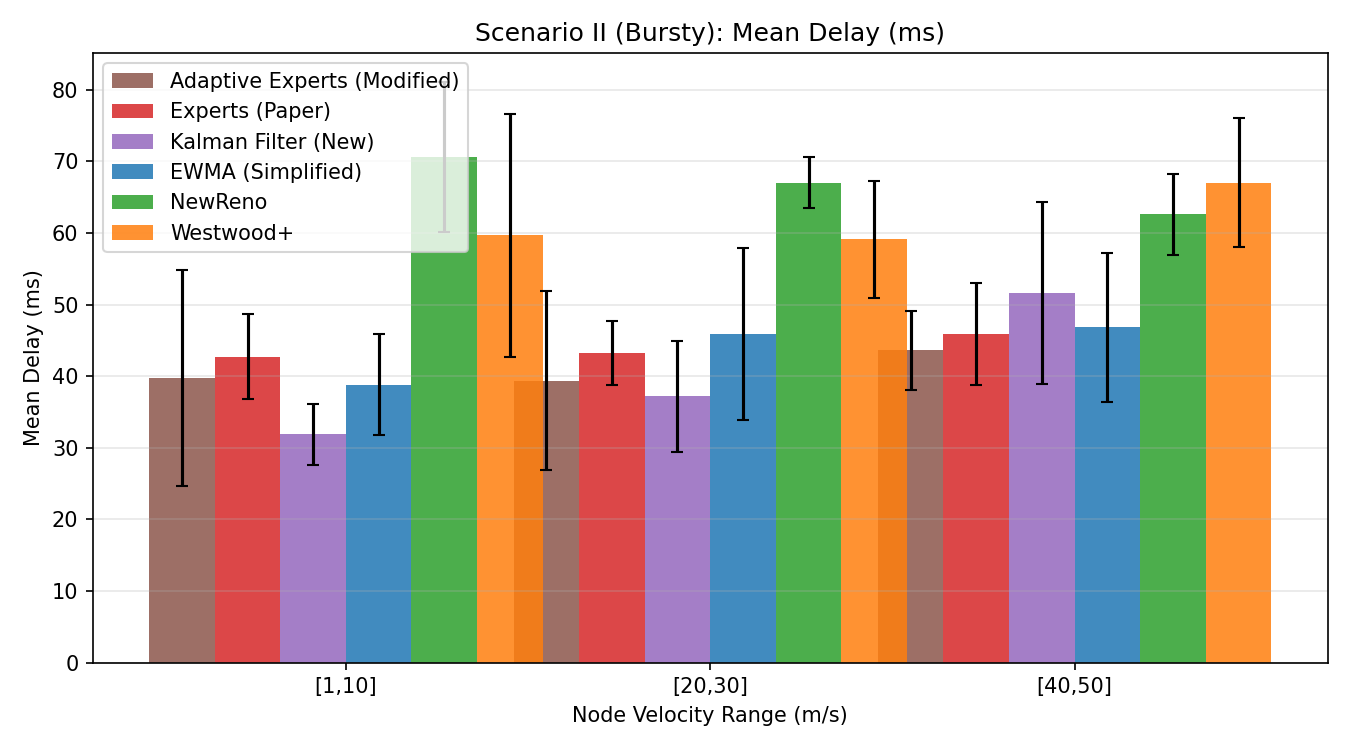
\includegraphics[width=\linewidth]{../results/scenario2/s2_delay.png}
        \caption{Scenario II Delay}
    \end{subfigure}
    \hfill
    \begin{subfigure}{0.48\textwidth}
        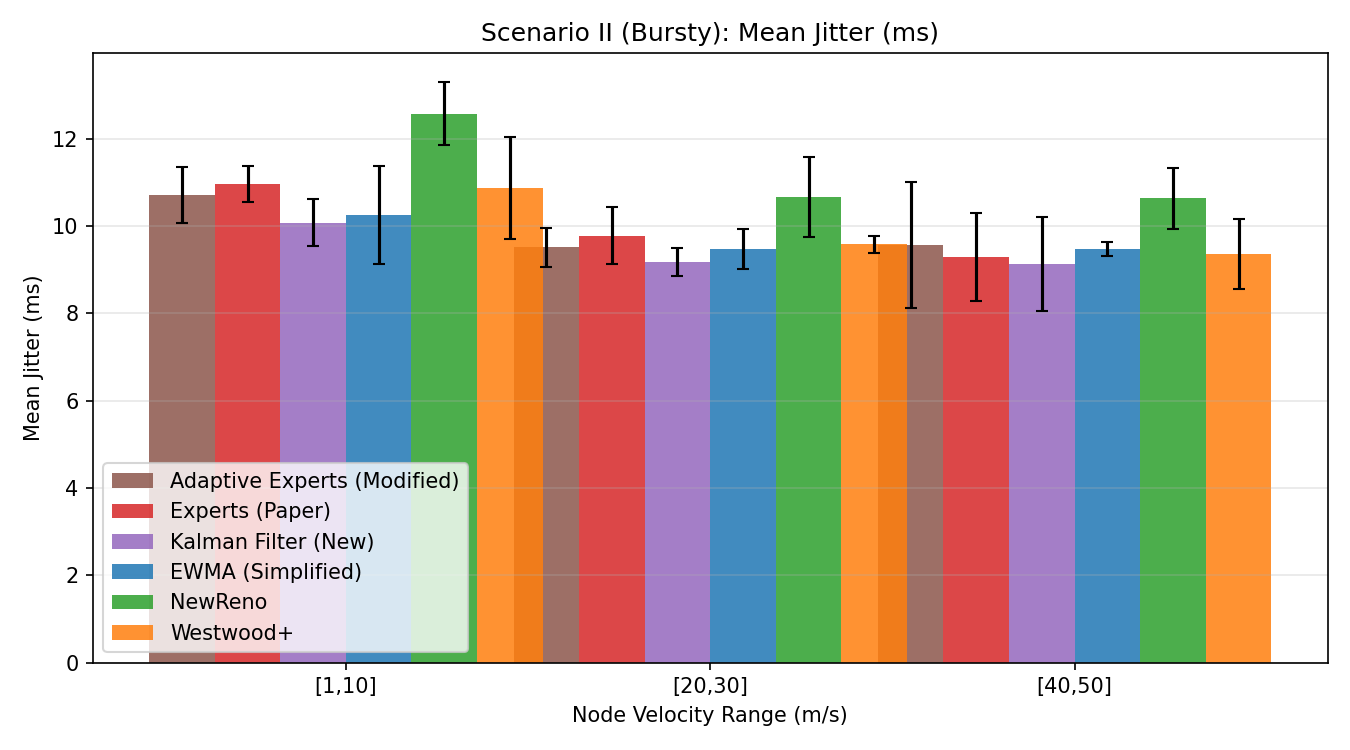
\includegraphics[width=\linewidth]{../results/scenario2/s2_jitter.png}
        \caption{Scenario II Jitter}
    \end{subfigure}
    \caption{Scenario II latency behavior}
\end{figure}

\begin{figure}[H]
    \centering
    \begin{subfigure}{0.48\textwidth}
        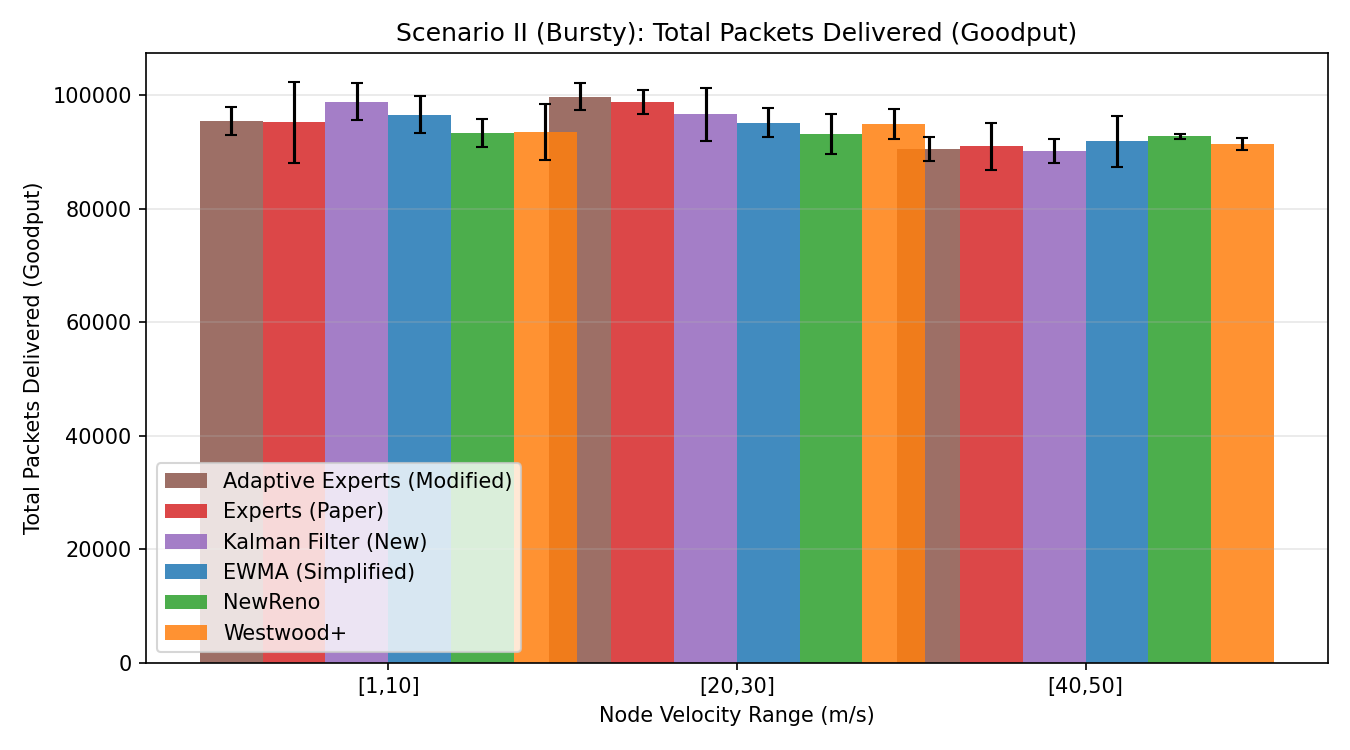
\includegraphics[width=\linewidth]{../results/scenario2/s2_goodput.png}
        \caption{Scenario II Goodput}
    \end{subfigure}
    \hfill
    \begin{subfigure}{0.48\textwidth}
        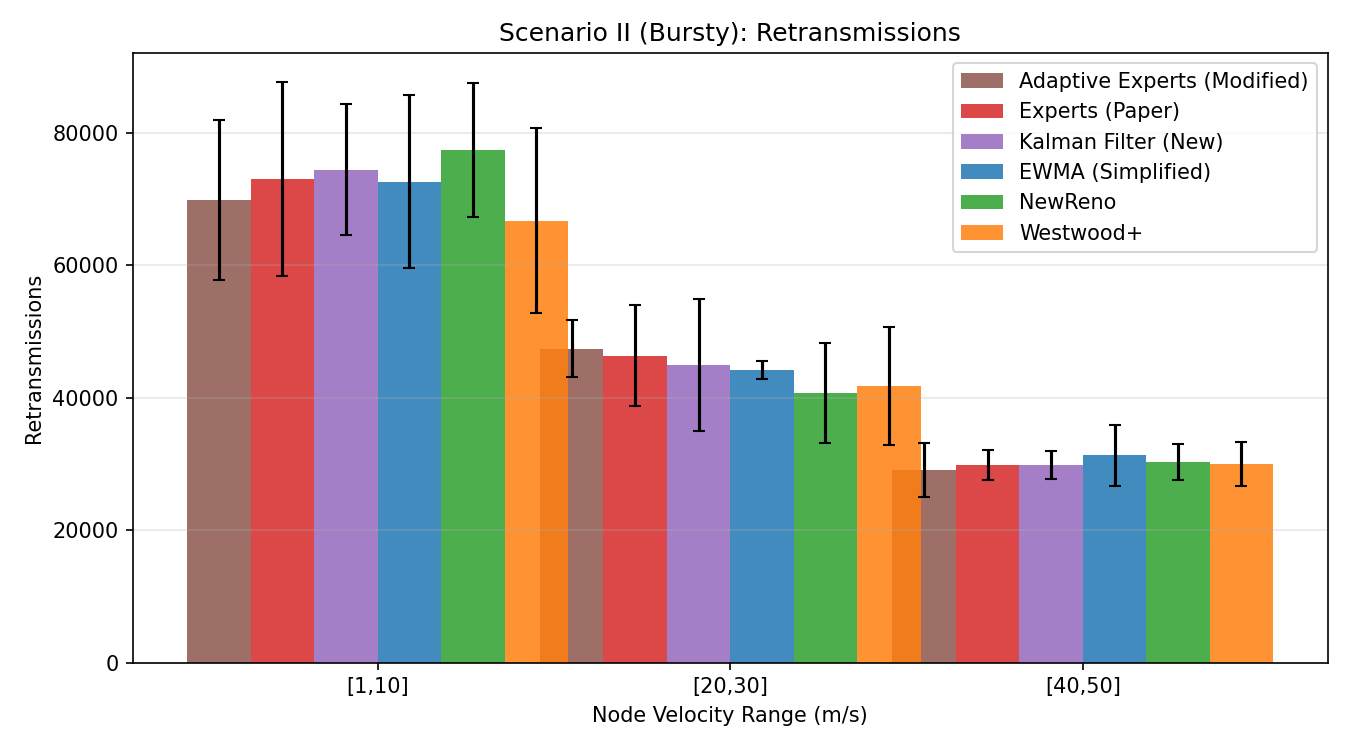
\includegraphics[width=\linewidth]{../results/scenario2/s2_retransmissions.png}
        \caption{Scenario II Retransmissions}
    \end{subfigure}
    \caption{Scenario II efficiency and retransmission comparison}
\end{figure}

\section{Discussion}
\textbf{Key observations:}
\begin{itemize}
    \item ML-based variants (Experts/Adaptive/Kalman/EWMA) generally maintain lower delay than NewReno/Plus in bursty conditions, reflecting more conservative RTT-aware behavior.
    \item Kalman is the strongest low-delay alternative overall among non-paper variants.
    \item Adaptive Experts currently matches Experts in the evaluated short-run setup, indicating the modification is behavior-preserving under these operating conditions.
    \item Baseline NewReno and Plus can achieve higher throughput in Scenario II, but with noticeably higher delay and/or loss.
\end{itemize}

\textbf{Why Adaptive and Experts can match:}
\begin{itemize}
    \item Short duration and limited seeds can reduce exposure to large regime switches.
    \item Adaptive terms may stay near base values if innovation remains moderate.
    \item Parameter sensitivity ($\beta,\gamma,\mu,W$) likely requires dedicated sweeps.
\end{itemize}

\section{Threats to Validity}
\begin{itemize}
    \item Short-mode experiment length (300s/600s) is useful for iteration but not as strong as full paper durations.
    \item Three seeds are adequate for trend exploration, but confidence intervals improve with larger seed sets.
    \item Scenario assumptions (traffic mix, mobility ranges, packet size) can influence ranking.
\end{itemize}

\section{Reproducibility}
\begin{verbatim}
./ns3 build
bash tools/run_scenario1.sh short
bash tools/run_scenario2.sh short
python3 tools/analyze_scenarios.py
\end{verbatim}

Primary outputs:
\begin{itemize}
    \item \texttt{results/scenario1/scenario1\_results.csv}
    \item \texttt{results/scenario1/scenario1\_aggregated.csv}
    \item \texttt{results/scenario2/scenario2\_results.csv}
    \item \texttt{results/scenario2/scenario2\_aggregated.csv}
    \item Plots in \texttt{results/scenario1/} and \texttt{results/scenario2/}
\end{itemize}

\section{Conclusion}
This project delivers a full, reproducible ns-3 research framework for ML-enhanced TCP RTT prediction and congestion control. It includes paper algorithm reproduction, modified paper algorithm design, alternative online predictors, complete scenario automation, and publication-style analysis outputs. The implementation demonstrates that RTT-aware control can provide improved latency behavior in challenging wireless settings, while throughput-latency trade-offs remain workload dependent.

\section*{Acknowledgment of Source Algorithm}
The original Fixed-Share Experts idea follows Nunes et al. (ICCCN 2011). This report's Adaptive Experts, EWMA simplification, and Kalman-based variant are implementation extensions for comparative study in ns-3.

\end{document}
